\section{Complex Numbers}

\begin{mainbox}{General}

    $z = \underbrace{x}_\text{\textcolor{red}{Re}} +\:i\underbrace{y}_\text{\textcolor{red}{Im}} = \underbrace{r \cdot (\cos(\varphi) + i \cdot \sin(\varphi)) = r \cdot e^{i\varphi}}_\text{\textcolor{red}{Polarform}}\\
    \compconj{z} = x - iy = r \cdot e^{i(2\pi - \varphi)}\\
    |z| = r = \sqrt{x^{2} + y^{2}} = \sqrt{z \cdot \compconj{z}}\\
    \varphi = \begin{cases}
        arc tan(\frac{y}{x}), &\RN{1}\:Q.\\
        arc tan(\frac{y}{x}) + \pi, &\RN{2}/\RN{3}\:Q.\\
        arc tan(\frac{y}{x}) + 2\pi, &\RN{4}\:Q.\\
    \end{cases}$

\end{mainbox}
\begin{mainbox}{Operations}
\setlength{\tabcolsep}{2pt}
    \begin{tabular}{rl}
        $+/-:$ & $(x_{1} + x_{2}) + (y_{1} + y_{2})i$ \\
        $z_1\cdot z_2:$ & $(x_{1} + y_{1}i)(x_{2} + y_{2}i) = r_{1}\cdot r_{2}\cdot e^{i(\varphi_{1} + \varphi_{2})}$ \\
        $\frac{z_{1}}{z_{2}}:$ & $\frac{z_1\cdot\compconj{z}_2}{|z_2|^2} = \frac{r_{1}}{r_{2}}\cdot e^{i(\varphi_{1} - \varphi_{2})}$ \\
        $z^n:$ & $r^n\cdot e^{i\varphi n}$ \\
        $\sqrt{a}:$ & $a = z^n  \Leftrightarrow |a|\cdot e^{i\alpha} = r^n\cdot e^{i\varphi n} \underset{k = 0,...,n-1}{\begin{cases}
            r = \sqrt[n]{|a|} \\
            \varphi = \frac{\alpha + 2k\pi}{n}
        \end{cases}}$
    \end{tabular}
\end{mainbox}
\begin{mainbox}{Polynomials}
\setlength{\tabcolsep}{2pt}
    \begin{tabular}{rl}
        degree 2: & $z = \frac{b\pm \sqrt{b^2 - 4ac}}{2a}$\\
        special case: & $az^n + c = 0 \Leftrightarrow z = \sqrt[n]{-\frac{c}{a}}$
    \end{tabular}    
\end{mainbox}
\begin{mainbox}
    \text{With polynomials with complex roots, the roots occur as a complex-conjugate pair.}
    \smallskip\\
    \text{Polynomials over} $\mathbb{C}$ \text{with an odd degree}\\
    \text{have at least one root in} $\mathbb{R}$.
\end{mainbox}
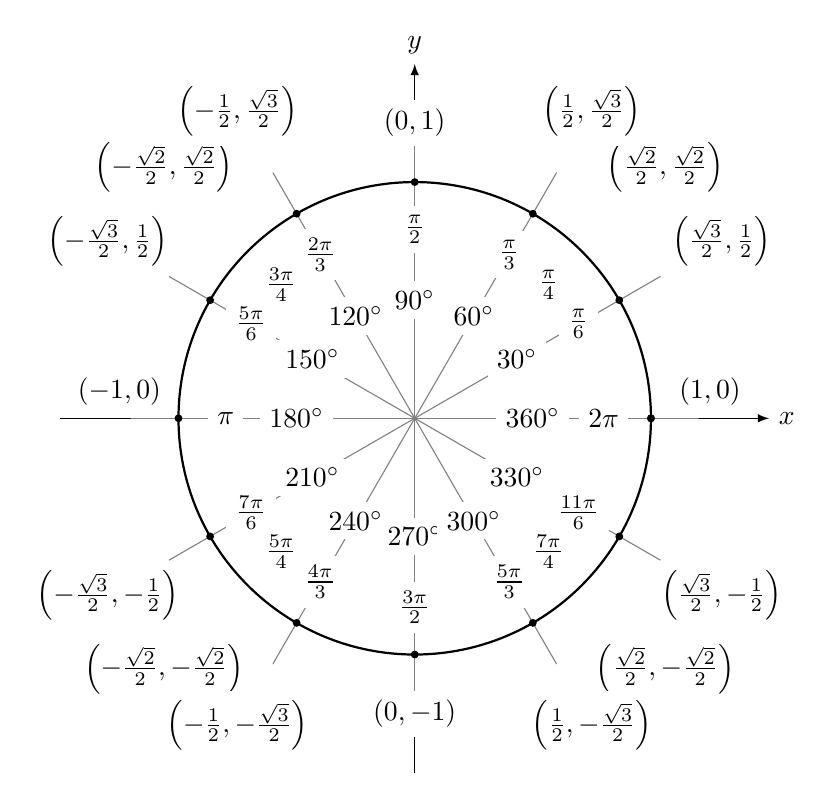
\begin{tikzpicture}[scale=3,cap=round,>=latex]
        % draw the coordinates
        \draw[->] (-1.5cm,0cm) -- (1.5cm,0cm) node[right,fill=white] {$x$};
        \draw[->] (0cm,-1.5cm) -- (0cm,1.5cm) node[above,fill=white] {$y$};

        % draw the unit circle
        \draw[thick] (0cm,0cm) circle(1cm);

        \foreach \x in {0,30,...,360} {
                % lines from center to point
                \draw[gray] (0cm,0cm) -- (\x:1.2cm);
                % dots at each point
                \filldraw[black] (\x:1cm) circle(0.4pt);
                % draw each angle in degrees
                \draw (\x:0.5cm) node[fill=white] {$\x^\circ$};
        }

        % draw each angle in radians
        \foreach \x/\xtext in {
            30/\frac{\pi}{6},
            45/\frac{\pi}{4},
            60/\frac{\pi}{3},
            90/\frac{\pi}{2},
            120/\frac{2\pi}{3},
            135/\frac{3\pi}{4},
            150/\frac{5\pi}{6},
            180/\pi,
            210/\frac{7\pi}{6},
            225/\frac{5\pi}{4},
            240/\frac{4\pi}{3},
            270/\frac{3\pi}{2},
            300/\frac{5\pi}{3},
            315/\frac{7\pi}{4},
            330/\frac{11\pi}{6},
            360/2\pi}
                \draw (\x:0.8cm) node[fill=white] {$\xtext$};

        \foreach \x/\xtext/\y in {
            % the coordinates for the first quadrant
            30/\frac{\sqrt{3}}{2}/\frac{1}{2},
            45/\frac{\sqrt{2}}{2}/\frac{\sqrt{2}}{2},
            60/\frac{1}{2}/\frac{\sqrt{3}}{2},
            % the coordinates for the second quadrant
            150/-\frac{\sqrt{3}}{2}/\frac{1}{2},
            135/-\frac{\sqrt{2}}{2}/\frac{\sqrt{2}}{2},
            120/-\frac{1}{2}/\frac{\sqrt{3}}{2},
            % the coordinates for the third quadrant
            210/-\frac{\sqrt{3}}{2}/-\frac{1}{2},
            225/-\frac{\sqrt{2}}{2}/-\frac{\sqrt{2}}{2},
            240/-\frac{1}{2}/-\frac{\sqrt{3}}{2},
            % the coordinates for the fourth quadrant
            330/\frac{\sqrt{3}}{2}/-\frac{1}{2},
            315/\frac{\sqrt{2}}{2}/-\frac{\sqrt{2}}{2},
            300/\frac{1}{2}/-\frac{\sqrt{3}}{2}}
                \draw (\x:1.5cm) node[fill=white] {$\left(\xtext,\y\right)$};

        % draw the horizontal and vertical coordinates
        % the placement is better this way
        \draw (-1.25cm,0cm) node[above=1pt] {$(-1,0)$}
              (1.25cm,0cm)  node[above=1pt] {$(1,0)$}
              (0cm,-1.25cm) node[fill=white] {$(0,-1)$}
              (0cm,1.25cm)  node[fill=white] {$(0,1)$};
\end{tikzpicture}


